\section{LLVM 中如何实现这个算法}


\begin{frame}
    \frametitle{TL; DR}

    算法主体主要实现在 lib/CodeGen/MachineBlockPlacement.cpp

    \vspace{1.5em}

    其中分支概率等信息来源于 Block\{Frequency, ProbabilityInfo\}

    \vspace{1.5em}

    各个 Target 需要实现 \{ analyze, insert, remove \}Branch等虚函数,RISC-V在 5 年前,D40808\cite{llvmriscvimplbranchanalysis2017}实现;两年前,D84833包含了一个间接分支实现 \cite{llvmriscvimplindirect2020}
    \begin{table}
        \begin{tabular}{ccc}
            \toprule
            功能   & 实现                    & 源代码位置                                                                              \\
            \midrule
            边权   & BlockFrequency        & \cite{llvmblockfreqinfoimpl2022}                                                   \\
            块放置  & MachineBlockPlacement & buildCFGChains()\cite{llvmmachineblockplacement2022}                               \\
            块对齐  & MachineBlockPlacement & alignBlocks()\cite{llvmmachineblockplacement2022}                                  \\
            分支分析 & RISCVInstrInfo        & analyzeBranch()\cite{llvmriscvinstrinfo2022}\cite{llvmriscvimplbranchanalysis2017} \\
            \bottomrule
        \end{tabular}
        \caption{各个功能的实现情况和所在的位置}
    \end{table}

\end{frame}


\begin{frame}
    \frametitle{BOLT - Binary optimization and layout tool}

    Facebook 在 2018 年开源了他们的二进制优化工具 -- BOLT\cite{facebook2018bolt}。这个仓库现在已经合并到 LLVM,可以在对编译后的二进制进行基本的重排,冷热代码分离等工作。

    \begin{figure}
        \centering
        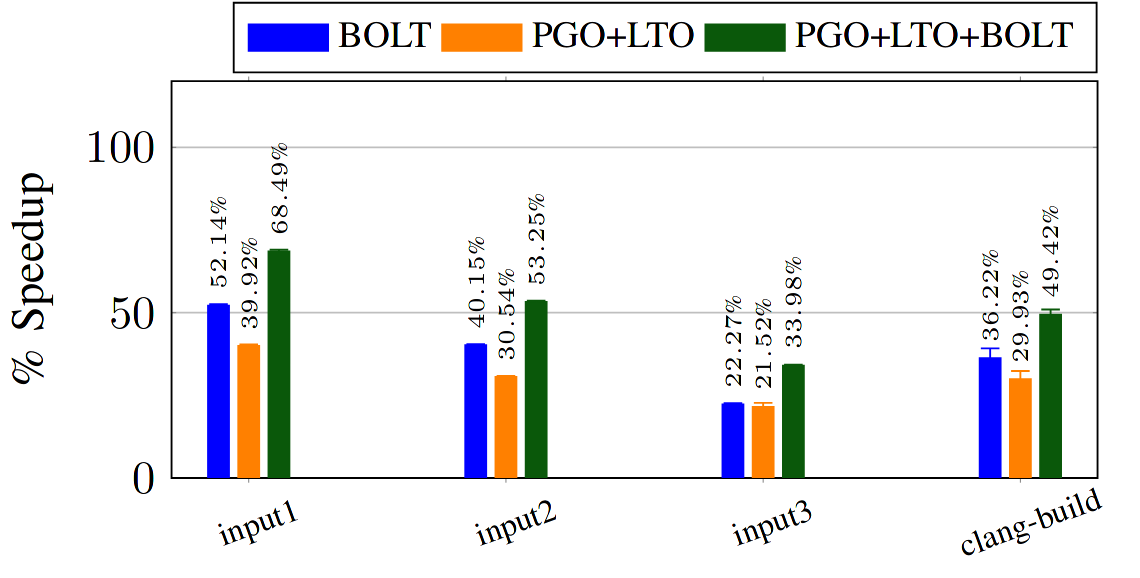
\includegraphics[width=0.6\textwidth]{images/perf_improv_clang.png}
        \caption{优化后的Clang}
    \end{figure}

\end{frame}